\title{Introduction to Data Analysis with \textsf{R}}
\author[T. Hothorn]{Torsten Hothorn}
\institute{
  Universit\"at Z\"urich \\
  \texttt{Torsten.Hothorn@R-project.org}
}

\date{}

\begin{document}

\frame{\titlepage}

\setbeamertemplate{footline}[page number]

\begin{frame}[fragile]

    \begin{columns}

       \begin{column}{3.5cm}
           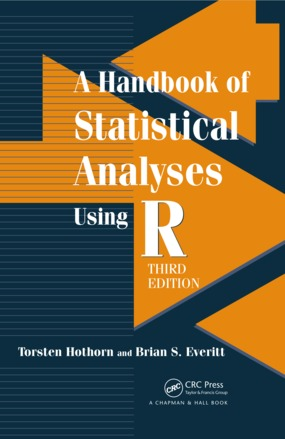
\includegraphics[width = 3cm]{graphics/HSAUR}
       \end{column}

       \begin{column}{7.5cm}

           This course material is based on 
           \booktitle{A Handbook of Statistical Analysis Using \R{}}
           (3rd edition) published by CRC press. 

           The \R{} package \Rpackage{HSAUR3} contains all data sets, 
           examples and \R{} code and is available from \curl{http://CRAN.R-project.org/package=HSAUR3}
       \end{column}
    \end{columns}

\end{frame}

